\frame{\frametitle{PCU Communication}
\begin{itemize}
\item Collective, unstructured exchanges
\item Each rank sends messages to local but
unstructured neighborhood
\item Buffer all messages between each pair
\item Exchange all messages between all pairs in one collective
\item However, communication graph is not known
\item Non-blocking send/receive (one per pair)
\item Non-blocking barrier for termination detection
\end{itemize}
}

\frame{\frametitle{PCU Threading}
\begin{itemize}
\item Treated like nested \texttt{mpiexec}
\item Thread has 3D contiguous mesh partition
\item Create/join through pthread
\item Uniform threads per process
\item Communication between threads
\item All threads have globally unique ranks
\item Can be compatible with other thread
managers by accepting their threads
\end{itemize}
}

\frame{\frametitle{PCU Threading}
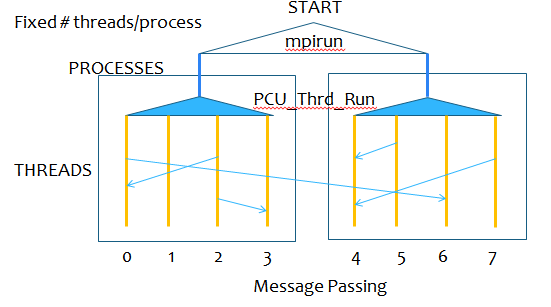
\includegraphics[width=0.8\textwidth]{threads.png}
}

\frame{\frametitle{Array Mesh Storage}
\begin{itemize}
\item Array-based structure that allows constant-time
insertion/removal and persistent indices
\item Linked lists in arrays encode variable-length data
\item Can represent unstructured meshes and efficiently
support adaptivity
\item 4X memory reduction
\item Much better data locality guarantees
\item Easier to allocate in possibly more restrictive future
memory architectures
\item Easier to serialize, indices not invalidated by
array relocation
\item More compatible with analysis structures
\end{itemize}
}
